\documentclass[12pt,a4paper,openany]{book}
%------------------------------------------------------------------------------------------------------------------------------------------------------------------------------------------------------------------------------
% PACKAGES
%--------------------------------------------------------------------------------------------------------------------------------------------------------------------------------------------------------------------------------

% Selección de idioma
\usepackage[spanish]{babel}

% algo
\usepackage[utf8]{inputenc}

% Par acomodar la foto del editorial
\usepackage{wrapfig}

% Paquetes útiles
\usepackage[table]{xcolor}
\usepackage{amssymb}
\usepackage{amsmath}
%\usepackage{mathbbol}
\usepackage{bbm}
\usepackage{amsthm}
\usepackage{pdfpages}
\usepackage{graphicx,color,psfrag}
\usepackage{epstopdf}
\usepackage{pdflscape}
\usepackage{tabularx}
\usepackage{longtable}
\usepackage{breakurl}
\usepackage{enumitem}
\usepackage[normalem]{ulem}
\usepackage{blindtext}
\usepackage{mathtools,breqn}

\usepackage{fnpct}

\usepackage{subcaption}

\usepackage{newpxtext}

% La mejor fuente de la letra: https://www3.gobiernodecanarias.org/medusa/ecoblog/lortrodm/files/2015/03/tarea-formatos-word.pdf
% caption fonts
%\usepackage[font={large,bf}]{caption} 
\usepackage[T1]{fontenc}
\usepackage{verdana}


\usepackage{setspace}
\usepackage{longtable}
\usepackage{threeparttable}  
\usepackage{tabulary}
\usepackage{booktabs}
\usepackage{float}
\usepackage{caption}
\usepackage{subcaption}
\usepackage{rotating}
\usepackage[titletoc,title]{appendix}

\usepackage{array,multirow}

\usepackage[round]{natbib}
\bibpunct{(}{)}{;}{a}{,}{;}
\setcounter{MaxMatrixCols}{10}

\topmargin=-1.8cm \textheight=23.8cm \oddsidemargin=-0.3cm
\evensidemargin=-0.5cm \textwidth=17.1cm

\newtheorem{theorem}{Theorem}
\newtheorem{corollary}[theorem]{Corollary}
\newtheorem{proposition}{Proposition}
\newtheorem{assumption}{Assumption}
\newtheorem{assumption2}{Assumption A}

\newtheorem{lemma}{Lemma}

\usepackage{tikz}
\usetikzlibrary{positioning}
\tikzset{>=stealth}
\usepackage{amsmath}
\usepackage{verbatim}
\usetikzlibrary{arrows,shapes}

% Definir colores
\definecolor{mycolor1}{RGB}{236, 244, 244}
\definecolor{mycolor2}{RGB}{164, 92, 92}	
\definecolor{mycolor3}{RGB}{252, 196, 108}
\definecolor{mycolor4}{RGB}{76, 60, 52}
\definecolor{mycolor5}{RGB}{164, 248, 208}
\definecolor{mycolor6}{RGB}{116, 112, 112}
\definecolor{mycolor7}{RGB}{116, 116, 52}
\usepackage[colorlinks=true,linkcolor=myblue, allcolors=mycolor2]{hyperref}
\usepackage{soul}

% Tablas
\usepackage{tabularx}
\usepackage{multirow}
\usepackage{multicol} 
\usepackage{booktabs}%\usepackage{booktabs, calc} %This is the package to use to have nice-looking tables. More documentation on the tables in LateX: https://www.tug.org/pracjourn/2007-1/mori/mori.pdf
\usepackage{threeparttable} 

\usepackage{lmodern}
\usepackage{booktabs}
\usepackage{pgfplots}

\graphicspath{{../figuras/}}

\begin{document}
	
	%---------------------------------------------------------------------------
	% TITLE PAGE
	%---------------------------------------------------------------------------
	\doublespacing
	
	\title{Boletín COVID-19}
	\author{Autores}
	
	\date{}

	%\maketitle
	
	
	%\thispagestyle{empty}\baselineskip1.385\baselineskip \newpage{}
	
	\pagestyle{plain}\pagenumbering{arabic}
	
	%insertar el cover
	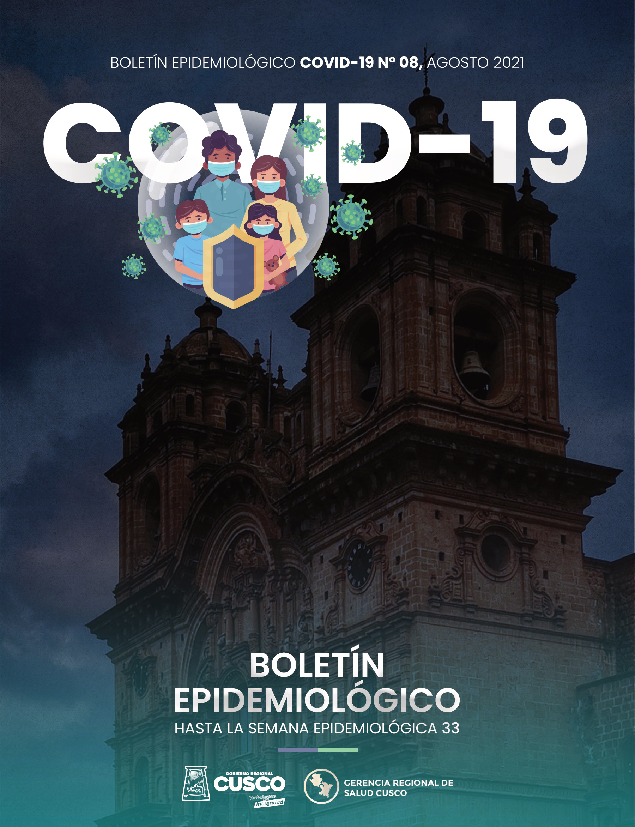
\includepdf[pages={1}]{../editorial/cover_boletin_8.pdf}
	\clearpage
	
	\pagestyle{plain}\pagenumbering{arabic}
	
	\clearpage
	
	
	\begin{center}
		{\large Gerencia Regional de Salud}
		
		\textbf{MSP. Javier Ramírez Escóbar}
		
		Gerente Regional \vspace{1.0cm}
		
		Dirección Ejecutiva de Inteligencia Sanitaria
		
		\textbf{MSP. Darío Francisco Navarro Mendoza}
		
		Director
		
		\vspace{1.5cm}
\noindent
\begin{minipage}[t]{.45\textwidth}
	\centering
	Dirección de Epidemiología e Investigación  \\
	\textbf{MSC. Fátima R. Concha Velasco}\\
	Directora \vspace{1.0cm}\\
	% Por orden alfabético del apellido
	\textit{Equipo de Epidemiología e Investigación }\vspace{.5cm}\\
	Econ. Karen Yorka Aguilar Zuñiga \\
	M.C Edwards Adrian Aguirre Valenzuela \\
	Lic. Nadia Isabel Cáceres Pillco \\
	Econ. Johar Jurimao Cassa Avendaño \\
	TAP. Edgar Waldo Capcha Salcedo \\
	M.S.P. Pablo Fidel Grajeda Ancca \\
	M.C. Katia Luque Quispe \\
	M.C. Ana Gabriela Eulalia Moncada Arias \\
	Lic. Enf. Ruth Nelly Oscco Abarca \\
	Lic. Enf. Guinetta Margarita Yabar Herrera \vspace{1.5cm}\\	
\end{minipage}
\hfill
\noindent
\begin{minipage}[t]{.45\textwidth}
	\centering
	Dirección de Estadística, Informática y Telecomunicaciones\\
	\textbf{Ing. Abel Rimasca Chacón} \\
	Director \vspace{1.0cm} \\
	% Por orden alfabético del apellido
	\textit{Equipo de Estadística, Informática y Telecomunicaciones} \vspace{.5cm} \\
	Ing. Iván Atayupanqui Rondón \\
	Ing. Miguel Ángel Campana Alarcón \\
	Ing. Uriel Lacuta Farfán \\
	Ing. Jorge Fernando Lovatón Ramos \\
	Ing. Danny Robert Moscoso Sánchez \\
	Lic. Ray Milton Valderrama Álverez \vspace{1.5cm}\\
\end{minipage}
Secretaria: Sra. Ruth Baca Mendoza
	\end{center}
\let\cleardoublepage\clearpage
	\tableofcontents
	\listoffigures
	\listoftables
	
	%\mainmatter
	%---------------------------------------------------------------------------
	% CAPÍTULO: EDITORIAL
	%---------------------------------------------------------------------------
	
	\chapter*{Editorial}
	\addcontentsline{toc}{chapter}{Editorial}
	
	\begin{wrapfigure}{l}{8.5cm}
		\label{wrap-fig:1}
		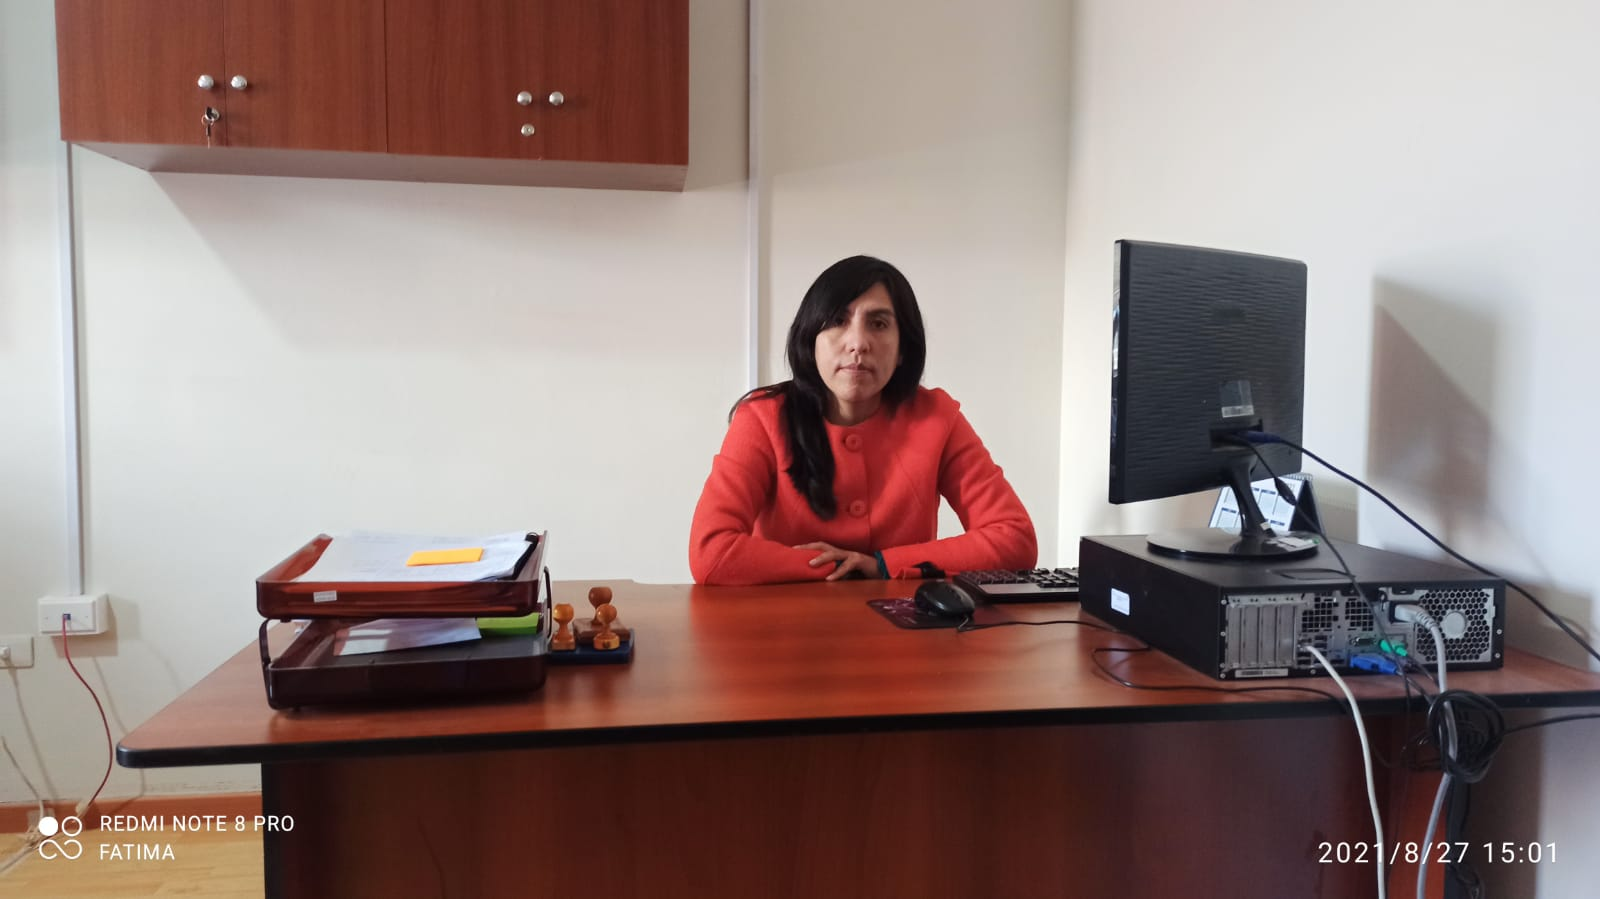
\includegraphics[width=8.5cm]{../editorial/foto_editorial.jpeg}
		\caption*{
			\centering
				MSC. Fátima Rosario Concha Velasco
				
				\textit{Directora de Epidemiología e Investigación}
				
				GERESA, Cusco }
	\end{wrapfigure}
	
	\noindent Un nuevo coronavirus, el SARS-CoV-2, apareció en diciembre del 2019, cuya transmisión a través del contacto directo o gotitas respiratorias dependiendo del tiempo y contacto cercano es más fácil y rápida en relación a los otros coronovarius. El virus se propagó rápidamente por todo el mundo a través de los viajeros, generando a la vez un incremento de la mortalidad. Se reconoce que los números notificados son subestimaciones de los casos de infección reales, considerando a los individuos asintomáticos con COVID-19 que no fueron identificados y rastreados.
	A nivel mundial, los gobiernos y las agencias tomaron medidas para contener la propagación de COVID-19, con rutinas aplicadas para la atención sanitaria y el distanciamiento social. Aun así, estas estrategias tuvieron consecuencias, como la crisis económica por el cierre de negocios y el cese de labores en diversas industrias. La calidad de la educación se vio afectada, ya que muchas escuelas carecían de plataformas y servicios de red. Por lo cual, la necesidad de continuar con la reactivación económica, traduce fortalecer a la brevedad la vacunación para COVID-19 en todos los grupos etarios. Continuar con las recomendaciones comunitarias para el distanciamiento y uso de máscaras que incluyen la prevención combinada y control de la fuente para las personas sintomáticas y asintomáticas. Así como, continuar con la oportuna identificación y rastreo de contactos de sintomáticos y asintomáticos.
	La vacunación preventiva generalizada puede reducir costos y desempeñar un papel fundamental en la protección de las personas contra la infección por COVID-19, facilitando la reducción significativa de la transmisión dentro de la población del rebaño. La preocupación de depender de las vacunas “sólo S”, por la presencia de mutaciones en la proteína pico (S) del SARS-CoV-2, genera una selección de variantes de COVID-19, con la ausencia del anticuerpo del huésped para empujar sistemáticamente al virus en una dirección determinada, aumentando la transmisibilidad y competencia entre ellas que podrían afectar la neutralización por sueros convalecientes. Siendo necesario considerar tanto la magnitud del cambio en la neutralización de anticuerpos, así como la posibilidad de que muchas vacunas candidatas necesiten ser rediseñadas y probadas.  Sin embargo, hasta la fecha, la vacunación para COVID-19 aun es la mejor manera de combatir la infección por SARS-CoV-2. Se han aprobado 8 tipos de vacuna para ser aplicados entre grupos prioritarios bajo una autorización de uso de emergencia (EUA), incluida la vacuna Moderna mRNA-1273, vacuna Pfizer-BioNtech BNT162b2, China Las vacunas CoronaVac ™ y COVID-19 de Sinopharm, las vacunas Sputnik V y EpiVacCorona de Rusia, el nuevo coronavirus ChAdOx1 2019 de AstraZeneca (nCoV-19), y el Ad26.COV2.S. de Janssen.
	Por lo cual, a partir del conocimiento generado en la información de la situación actual de COVID-19 en la Región Cusco, es importante continuar fortaleciendo la vacunación para COVID-19, la cual como se ha mencionado es la principal herramienta en la lucha contra el COVID-19, ayudándonos a desarrollar inmunidad, protegiendo a las personas que nos rodean, principalmente a los que tienen más riesgo de complicaciones graves. Así como también, es necesario que se siga fortaleciendo la detección y rastreo oportuno de casos para facilitar el control de la transmisión de la enfermedad.
	
	%---------------------------------------------------------------------------
	% CAPÍTULO: METODOLOGÍA
	%---------------------------------------------------------------------------
	
	\chapter*{Metodología}
	\addcontentsline{toc}{chapter}{Metodología}
	\noindent El presente Boletín tiene el objetivo de informar sobre los principales indicadores epidemiológicos y de gestión hospitalaria,  para hacer el seguimiento de la pandemia en nuestra región y tomar mejores decisiones. Este Boletín tiene una metodología de tipo descriptiva. En él, se encuentra un análisis extensivo de la situación actual de la pandemia en nuestra región desde la semana epidemiológica (SE) 1 a la 38 del 2021 (3 de enero al 25 de septiembre).
	
	Los datos analizados incluyeron: a) características generales: sexo, edad, casos confirmados, fallecidos; b) características clínicas: manifestaciones clínicas, casos confirmados sintomáticos, casos confirmados asintomáticos y comorbilidades; c) indicadores epidemiológicos: sistema de vigilancia epidemiológica, tasa de mortalidad, tasa de positividad de pruebas diagnósticas, casos activos – recuperados, y exceso de muerte por todas las causas, y d) indicadores de gestión hospitalaria: , ocupación de camas UCI y No.UCI en la Región.
	
	Las fuentes de información son las bases de datos de NOTI WEB (aplicativo del Sistema de Vigilancia Epidemiológica - COVID-19), SISCOVID (Sistema Integrado para COVID-19), SINADEF (Sistema Informático Nacional de Defunciones) y Reporte de Disponibilidad de Camas de Hospitalización, Región Cusco - de Referencias y Contrarreferencias de la Dirección de Emergencias y Desastres de GERESA-Cusco.
	
	Se usaron frecuencias absolutas y relativas para la descripción de los datos cualitativos. Para la descripción de datos cuantitativos se calcularon tasas (mortalidad, pruebas diagnósticas, incidencia de casos), promedios (ocupación de camas hospitalarias, fallecidos por COVID y fallecidos por todas las causas). Para describir la tendencia se representaron los datos cuantitativos y frecuencias relativas en intervalos de 7 días (semana epidemiológica). En las variables de sistema de vigilancia epidemiológica (1 prueba por 100,000 habitantes) y ocupación de cama (adecuado, menor a $70\%$, moderado, entre $75$ a $90\%$ y limitado, más de $90\%$), siendo todos los puntos de referencia sugeridos por la Organización Mundial de la Salud. Para el análisis de exceso de mortalidad, se usó la metodología descrita por C. Giattino, H. Ritchie, M. Roser, E. Ortiz-Ospina, y J. Hasell en el artículo ``Excess mortality during the Coronavirus pandemic (COVID-19)''. Published online at OurWorldInData.org.
	
	La descripción de dichas variables se hace de manera regional y provincial. En la presente edición se hace una descripción de la tasa de incidencia, tasa de mortalidad, tasa de positividad por prueba molecular y antigénica, y exceso de defunciones de todas las provincias de nuestra región. El lector interesado en un análisis distrital de los casos y defunciones puede encontrar en los links correspondientes.
	
	La novedad en esta edición; se presenta un análisis sobre las variantes de COVID-19 en la región,  usando como fuente de información el Registro y Reporte de Resultados en Línea (NETLAB) del Laboratorio Referencial Regional Cusco. Además, se muestra una tabla con las provincias con cero defunciones semanales por COVID-19.
	
	%---------------------------------------------------------------------------
	% CAPÍTULO: CARACTERÍSTICAS GENERALES
	%---------------------------------------------------------------------------
		
	\chapter*{Características Generales}
	\addcontentsline{toc}{chapter}{Características Generales}
	
 	\noindent La cantidad de casos confirmados hasta el 25 de septiembre fue de 73,693. En la Figura \ref{fig:casos_edad_sexo} se divide la población en grupos de diez años. La mayor cantidad de casos está en la población de 30 a 39 años. En contraste, el grupo de población con menos casos fue el grupo de más de 90 años de edad y los de 0 a 9 años. La proporción de hombres y mujeres es bastante similar a lo largo de estos grupos de edad.
	
	\begin{figure}[h]
		\caption{Casos Confirmados de COVID-19 según Grupo de Edad y Sexo en la Región Cusco}\label{fig:casos_edad_sexo}
		\begin{center}
			\includegraphics[width=0.65\linewidth]{../figuras/figura1}
		\end{center}
		{\footnotesize {Fuente de datos: SISCOVID, NOTICOVID.}}
	\end{figure}
	La Figura  \ref{fig:fallecidos_edad_sexo}  muestra el número de muertes hasta la semana epidemiológica número 38, teniendo 2,909 defunciones por COVID-19. La mayor cantidad de defunciones está en el grupo de 70 a 79 años de edad. Le sigue el grupo de población de 60 a 69 años y el grupo de 50 a 59 años. Es interesante notar que la población de varones supera en defunciones por COVID-19 al de las mujeres a lo largo de (casi todos) los grupos de edad.
	\begin{figure}[h]
		\caption{Casos fallecidos por COVID-19 según grupo de edad y sexo en la región Cusco, hasta la SE 38, 2021}\label{fig:fallecidos_edad_sexo}
		\begin{center}
			\includegraphics[width=0.65\linewidth]{../figuras/figura2}
		\end{center}
		{\footnotesize {Fuente de datos: SISCOVID, NOTICOVID.}}
	\end{figure}
	
%---------------------------------------------------------------------------
% CAPÍTULO: CARACTERÍSTICAS CLÍNICAS
%---------------------------------------------------------------------------
	\chapter*{Características Clínicas}
	\addcontentsline{toc}{chapter}{Características Clínicas}	
	
	\noindent La Figura \ref{fig:manifestaciones_clinicas}  muestra que los dos síntomas más frecuentes por COVID-19, en la Región de Cusco, fueron la tos (15.9$ \% $) y el dolor de garganta (15.1$ \% $). En menor porcentaje (menos del 2$ \% $), los pacientes reportaron irritabilidad, dolor abdominal, y dolor articular. 

	\begin{figure}[h]
		\caption{Manifestaciones Clínicas en Pacientes con COVID-19 en la Región Cusco, hasta la SE 38, 2021 }\label{fig:manifestaciones_clinicas}
		\begin{center}
			\includegraphics[width=0.65\linewidth]{../figuras/figura3}
		\end{center}
		{\footnotesize {Fuente de datos: SISCOVID, NOTICOVID.}}
	\end{figure}


	En la Figura \ref{fig:sintomaticos_asintomati} se evidencia la curva epidémica de casos sintomáticos y asintomáticos desde el inicio de la pandemia. Para el 2021, desde la SE 20 a la SE 38 se evidenció una consistente disminución de casos sintomáticos y asintomáticos, ésta es persistente hasta la última semana de análisis.
	\medskip
	
	\begin{figure}[h]
	\caption{Casos Sintomáticos y Asintomáticos de COVID-19, por Semana Epidemiológica en la Región Cusco, hasta la SE 38, 2020-2021  }\label{fig:sintomaticos_asintomati}
	\begin{center}
		\includegraphics[width=0.65\linewidth]{../figuras/figura4}
	\end{center}
	{\footnotesize {Fuente de datos: SISCOVID, NOTICOVID.}}
	\end{figure}


	La Figura \ref{fig:comorbilidades} muestra que las comorbilidades más frecuentes fueron la obesidad y diabetes (26 $\%$ cada una) y la enfermedad cardiovascular (19.7 $\%$). Por lo tanto, el 72.2 $\%$ de las comorbilidades corresponden a estas tres mencionadas.
	
	\begin{figure}[h]
	\caption{Comorbilidades en COVID-19 de la Región Cusco, hasta la SE 38, 2021}\label{fig:comorbilidades}
	\begin{center}
		\includegraphics[width=0.65\linewidth]{../figuras/figura5}
	\end{center}
	{\footnotesize {Fuente de datos: SISCOVID, NOTICOVID.}}
	\end{figure}

	La Figura \ref{fig:sign} muestra que el signo más frecuente fue el exudado faríngeo (62.3 $\%$ ), seguido por la disnea (22.1 $\%$ ).
	
	\begin{figure}[h]
	\caption{Signos en Pacientes COVID-19 de la Región Cusco, hasta la SE 38, 2021}\label{fig:sign}
	\begin{center}
		\includegraphics[width=0.65\linewidth]{../figuras/figura5b}
	\end{center}{\footnotesize {Fuente de datos: SISCOVID, NOTICOVID.}}
	\end{figure}

%---------------------------------------------------------------------------
% CAPÍTULO: ANÁLISIS DE INDICADORES
%---------------------------------------------------------------------------
    \chapter*{Análisis de Indicadores}
    \addcontentsline{toc}{chapter}{Análisis de Indicadores}
   
	\noindent La Figura \ref{fig:vigilancia_regional} muestra que la tasa de toma de pruebas, para el sistema de vigilancia epidemiológica a nivel regional, se encuentra por encima del estándar establecido por la Organización Mundial de la Salud. En las semanas epidemiológicas 37 y 38 se registraron entre 2.09 y 1.98 pruebas por 1000 habitantes, respectivamente.
	
	\begin{figure}[h]
	\caption{Sistema de Vigilancia Regional, hasta la SE 38, 2021 }\label{fig:vigilancia_regional}
	\begin{center}
		\includegraphics[width=0.65\linewidth]{../figuras/figura6}
	\end{center}
	{\footnotesize {Fuente de datos: SISCOVID, NOTICOVID.}}
	\end{figure}

	\section*{Ocupación de Camas}
	\noindent En la Figura \ref{fig:ocupacion_uci}, se muestra el promedio total de camas UCI COVID-19, las que se han incrementado desde la SE 1 (23) hasta la SE 38 (39). El promedio de ocupación de camas se mantuvo en 100 $\%$ de ocupación desde la SE 14, superando el 90 $\%$, posteriormente en la semana 34 hubo una tendencia discreta al descenso llegando al porcentaje de ocupación más bajo en la semana 36 (81$\%$), siendo esta la cifra más baja observada durante el año 2021.
	
	\begin{figure}[h]
	\caption{Ocupación de Camas UCI COVID-19 en la Región Cusco, hasta la SE 38, 2021}\label{fig:ocupacion_uci}
	\begin{center}
		\includegraphics[width=0.65\linewidth]{../figuras/figura7}
	\end{center}
	{\footnotesize {Fuente de datos: REFERENCIAS Y CONTRAREFERENCIAS.}}
	\end{figure}

	En la Figura \ref{fig:ocupacion_3_nivel} se observa la disponibilidad y ocupación de camas de hospitalización por COVID-19, no correspondiente a UCI, en los hospitales de nivel III, ha incrementado desde la SE 1 (312) hasta la SE 38 (386). Desde la SE 19 se ha observado una tendencia decreciente en la ocupación de camas no UCI, con una ocupación del 18 $\%$ en la SE 38.
	
	\begin{figure}[h]
	\caption{Ocupación de Camas UCI COVID-19 en la Región Cusco, hasta la SE 38, 2021}\label{fig:ocupacion_3_nivel}
	\begin{center}
		\includegraphics[width=0.65\linewidth]{../figuras/figura8}
	\end{center}
	{\footnotesize {Fuente de datos: REFERENCIAS Y CONTRAREFERENCIAS.}}
	\end{figure}

	En la Figura \ref{fig:ocupacion_2nivel}, se muestra el número de camas de hospitalización por COVID-19, en los hospitales de nivel II, número que ha aumentado desde la SE 1 (185) hasta la SE 38 (251). Sin embargo, desde la SE 21 se ha observado una disminución en la ocupación de camas en hospitales del nivel II, llegando hasta el 12 $\%$ en la SE 38.
	
	\begin{figure}[h]
	\caption{Disponibilidad y Ocupación de Camas a Nivel de Hospitales del Nivel II en la Región Cusco, hasta la SE 38, 2021}\label{fig:ocupacion_2nivel}
	\begin{center}
		\includegraphics[width=0.65\linewidth]{../figuras/figura9}
	\end{center}
	{\footnotesize {Fuente de datos: REFERENCIAS Y CONTRAREFERENCIAS.}}
	\end{figure}

\clearpage

	\section*{Tasas de positividad}
	\noindent  La Figura \ref{fig:tasa_positividad} muestra que la tasa de positividad total aumentó desde la SE 1 (4 $\%$) a la SE 3 (27 $\%$). Luego se mantuvo con una tendencia horizontal con un mínimo de 21$\%$ y máximo de 29 $\%$ durante la SE 3 y SE 18. Tras o cual hubo un discreto incremento en la semana 19, llegando a alcanzar un 39 $\%$. A la SE 38, la tasa de positividad total cayó a 11 $\%$, siendo esta la cifra más baja registrada en los últimos 6 meses del año.

	\begin{figure}[h]
	\caption{Frecuencia de Positivos y Tasa de Positividad Total por COVID-19 en la Región Cusco, hasta la SE 38, 2021  }\label{fig:tasa_positividad}
	\begin{center}
		\includegraphics[width=0.65\linewidth]{../figuras/figura11a}
	\end{center}
	{\footnotesize {Fuente de datos: SISCOVID, NOTICOVID.}}
	\end{figure}

	La Figura \ref{fig:total_muestras_procesada} muestra el promedio diario de todas las pruebas procesadas por COVID-19, para el año 2021. El promedio para las 5 últimas semanas (línea entrecortada de color negro) es de 482, esta cifra fue la más baja registrada durante el año 2021.
 
	\begin{figure}[h]
	\caption{Muestras Totales Procesadas por COVID-19 en la Región Cusco, hasta la SE 38, 2021}\label{fig:total_muestras_procesada}
	\begin{center}
		\includegraphics[width=0.65\linewidth]{../figuras/figura11b}
	\end{center}
	{\footnotesize {Fuente de datos: SISCOVID, NOTICOVID.}}
	\end{figure}

	La Figura \ref{fig:positivos_serologia} muestra que la tasa de positividad por prueba rápida serológica presentó una tendencia creciente hasta la SE 3 (26$\%$). Desde entonces la tasa de positividad sigue en incremento llegando a alcanzar el 41$\%$ en la SE 38, con una pendiente en ascenso.

	\begin{figure}[h]
	\caption{Frecuencia de Positivos y Tasa de Positividad por Pruebas Rápidas Serológicas en la Región Cusco, hasta la SE 38, 2021   }\label{fig:positivos_serologia}
	\begin{center}
		\includegraphics[width=0.65\linewidth]{../figuras/figura11c}
	\end{center}
	{\footnotesize {Fuente de datos: SISCOVID, NOTICOVID.}}
	\end{figure}
 
	La Figura \ref{fig:procesadas_serologia} muestra el promedio diario de las pruebas procesadas rápidas por COVID-19 de las semanas epidemiológicas 1 a 38 para el 2021. El promedio para las últimas 5 semanas (línea 	entrecortada de color negro) es de 61. Así se puede ver que, la semana 37 y 38 están por debajo de este promedio con un total de 63 y 45 pruebas procesadas, respectivamente

	\begin{figure}[h]
	\caption{Muestras Serológicas Procesadas por COVID-19 en la Región Cusco, hasta la SE 38, 2021}\label{fig:procesadas_serologia}
	\begin{center}
		\includegraphics[width=0.65\linewidth]{../figuras/figura11d}
	\end{center}
	{\footnotesize {Fuente de datos: SISCOVID}}
	\end{figure}

	En la Figura \ref{fig:positivos_antigenicas} se observa la tasa de positividad para pruebas antigénicas, la cual presentó una tendencia creciente hasta la SE 14 (26$\%$). Posteriormente, presentó una tendencia decreciente, hasta alcanzar un 8$\%$ en la SE 32 cifra que se mantuvo constante hasta la semana 38.	
	\begin{figure}[h]
	\caption{Frecuencia de Positivos y Tasa de Positividad para Pruebas Antigénicas en la Región Cusco, hasta la SE 38, 2021}\label{fig:positivos_antigenicas}
	\begin{center}
		\includegraphics[width=0.65\linewidth]{../figuras/figura11d}
	\end{center}
	{\footnotesize {Fuente de datos: SISCOVID}}
	\end{figure}
\clearpage
	La Figura \ref{fig:defunciones_semanal} muestra las defunciones a causa de COVID-19 por semana epidemiológica desde el inicio de la pandemia. Algo interesante que notar en esta figura son los hitos de referencia. El primer hito corresponde a la semana SE 52 del 2020 que corresponde a la semana de navidad (línea punteada morada), el segundo hito corresponde a la semana de año nuevo (SE 1, 2021) (línea punteada morada). Se puede notar que, desde este último hito las defunciones aumentan significativamente. Los siguientes hitos corresponden a la Semana Santa y a las elecciones presidenciales en primera y segunda vuelta secuencialmente. Desde la SE15, se ha presentado un descenso en la curva de fallecidos. En la SE38 hay una cantidad de defunciones bastante baja comparado con semanas previas. Este descenso es persistente.

	\begin{figure}[h]
	\caption{Defunciones por COVID-19 en la Región Cusco por Semana Epidemiológica, hasta la SE 38, 2021}\label{fig:defunciones_semanal}
	\begin{center}
		\includegraphics[width=0.65\linewidth]{../figuras/figura12}
	\end{center}
	{\footnotesize {Fuente de datos: SINADEF}}
	\end{figure}

	En la Figura \ref{fig:mortalidad_edad} muestra las mortalidad semanal para las edades agrupadas en diez años. Lo que se muestra es la tendencia al descenso de las muertes por COVID-19 - ajustadas por la cantidad de población que pertenece a ese grupo de edad -.  Ésta tendencia ha seguido en el grupo de población más vulnerable por edad (los adultos mayores),y también en los más jóvenes.\\
	\begin{figure}[h]
	\caption{Mortalidad por COVID-19 por Grupos de Edad, hasta la SE 38, 2021}\label{fig:mortalidad_edad}
	\begin{center}
		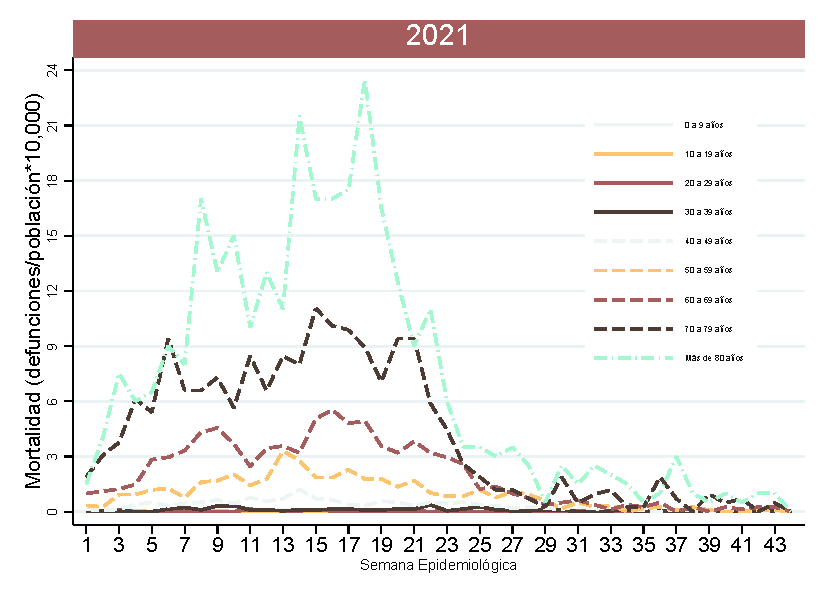
\includegraphics[width=0.65\linewidth]{../figuras/mortalidad_edad.pdf}
	\end{center}
	{\footnotesize Fuente de datos: SINADEF} 
	\end{figure}


	La Figura \ref{fig:mortalidad_grupo_edad} muestra la relación entre la tendencia de la mortalidad y las vacunas. Las líneas de referencia representan las fechas del inicio de las vacunas (primera y segunda dosis) para el correspondiente grupo de edad. Se espera, que la cobertura de vacunación ayude en disminuir la presentación del número de hospitalizados graves y fallecidos en eventuales futuras olas por COVID-19.

	\begin{figure}[h]
	\caption{Mortalidad por COVID-19 por Grupo de Edad, hasta la SE 38, 2021}
	\label{fig:mortalidad_grupo_edad}
	\centering
	\begin{subfigure}[b]{0.45\textwidth}
		\centering
		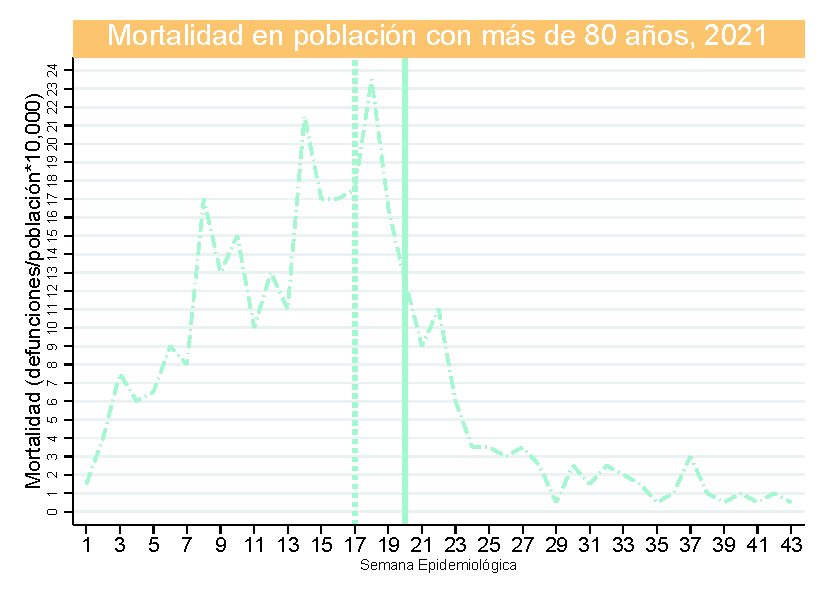
\includegraphics[width=\textwidth]{../figuras/mortalidad_edad_80.pdf}
		\caption{Más de 80 años}
		%\label{fig:}
	\end{subfigure}
	\hfill
	\begin{subfigure}[b]{0.45\textwidth}
		\centering
		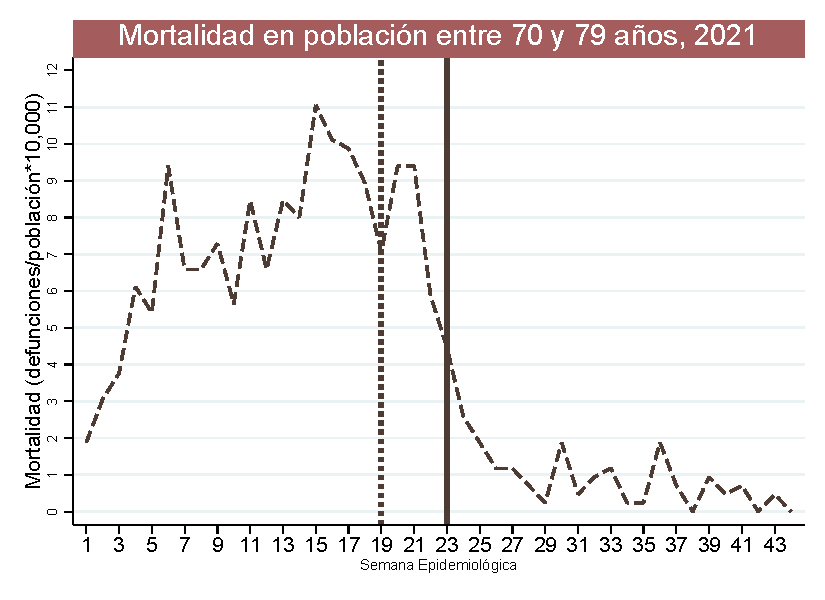
\includegraphics[width=\textwidth]{../figuras/mortalidad_edad_70.pdf}
		\caption{70 a 79 años}
		%\label{fig:70 a 79 años}
	\end{subfigure}

	\vspace{10mm}
	\begin{subfigure}[b]{0.45\textwidth}
		\centering
		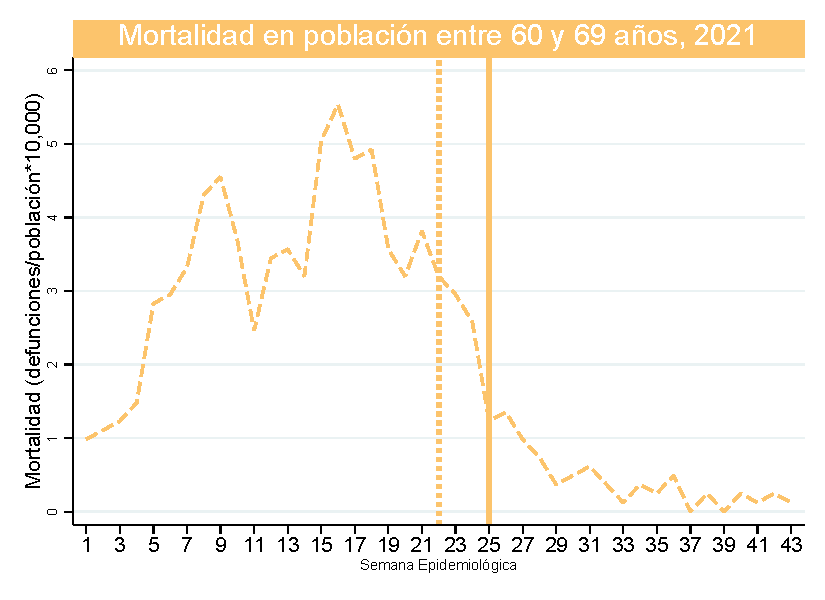
\includegraphics[width=\textwidth]{../figuras/mortalidad_edad_60.pdf}
		\caption{60 a 69 años}
		%\label{fig:60 a 69 años}
	\end{subfigure}
	\hfill
	\begin{subfigure}[b]{0.45\textwidth}
		\centering
		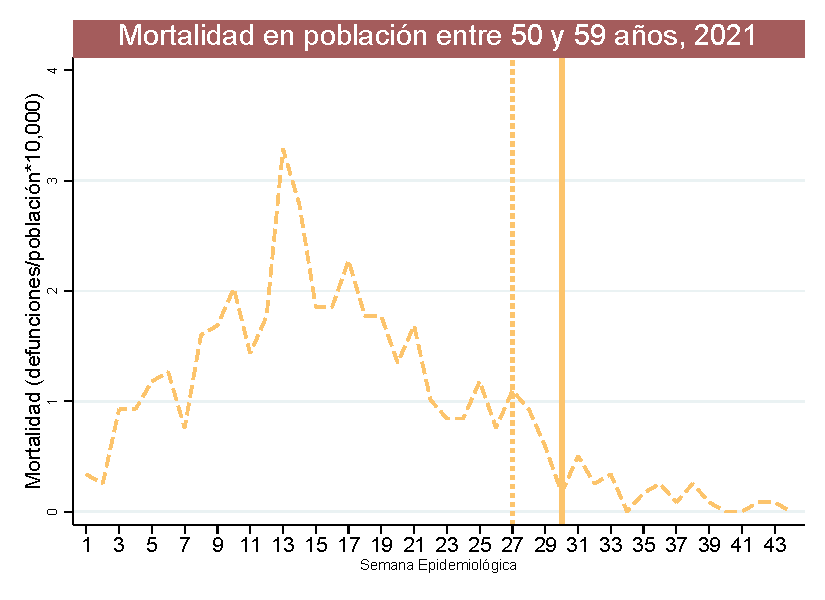
\includegraphics[width=\textwidth]{../figuras/mortalidad_edad_50.pdf}
		\caption{50 a 59 años}
		%\label{fig:50 a 59 años}
	\end{subfigure}

	\vspace{10mm}
	\begin{subfigure}[b]{0.45\textwidth}
		\centering
		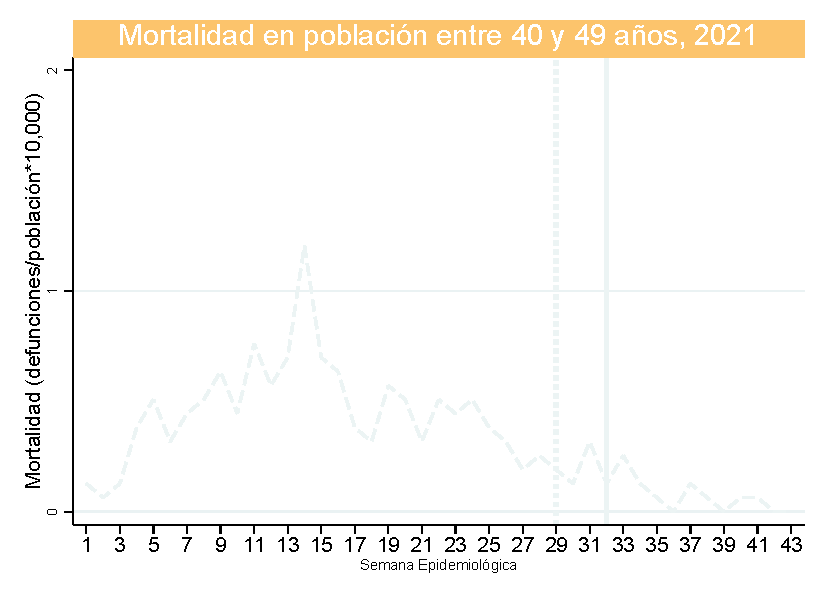
\includegraphics[width=\textwidth]{../figuras/mortalidad_edad_40.pdf}
		\caption{40 a 49 años}
		%\label{fig:40 a 49 años}
	\end{subfigure}
	\hfill
	\begin{subfigure}[b]{0.45\textwidth}
		\centering
		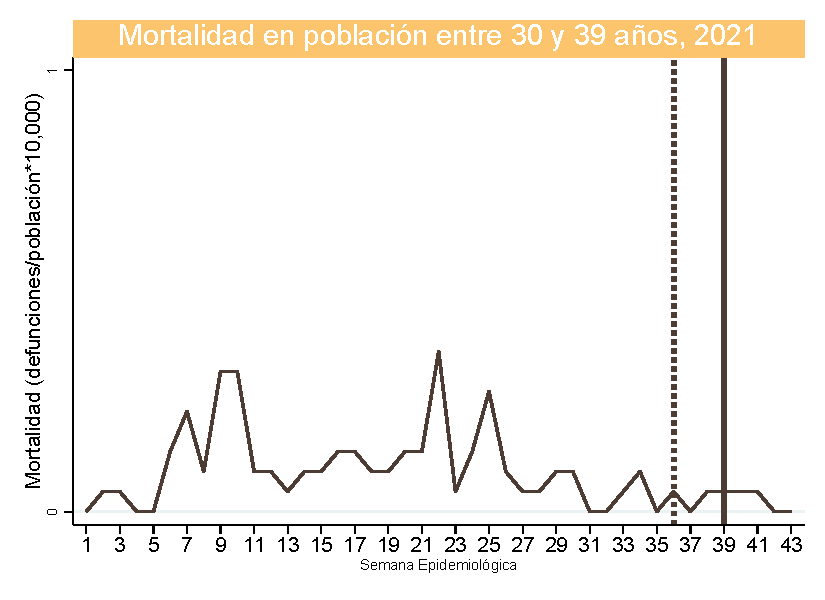
\includegraphics[width=\textwidth]{../figuras/mortalidad_edad_30.pdf}
		\caption{30 a 39 años}
		%\label{fig:40 a 49 años}
	\end{subfigure}
	\end{figure}

\clearpage
	
	\section*{Exceso de Muertes por Todas las Causas}
	\noindent  La Figura \ref{fig:exceso_regional} muestra que, a nivel regional, el exceso de defunciones por todas las causas ha disminuido en las últimas semanas. Para la SE 33 se registra un exceso de 0 fallecidos (no hay exceso) respecto al año 2019, cifra bastante menor a las semanas previas.

	\begin{figure}[h]
	\caption{Exceso de Fallecidos por  Todas las Causas, Región Cusco hasta la SE 38, 202}\label{fig:exceso_regional}
	\begin{center}
		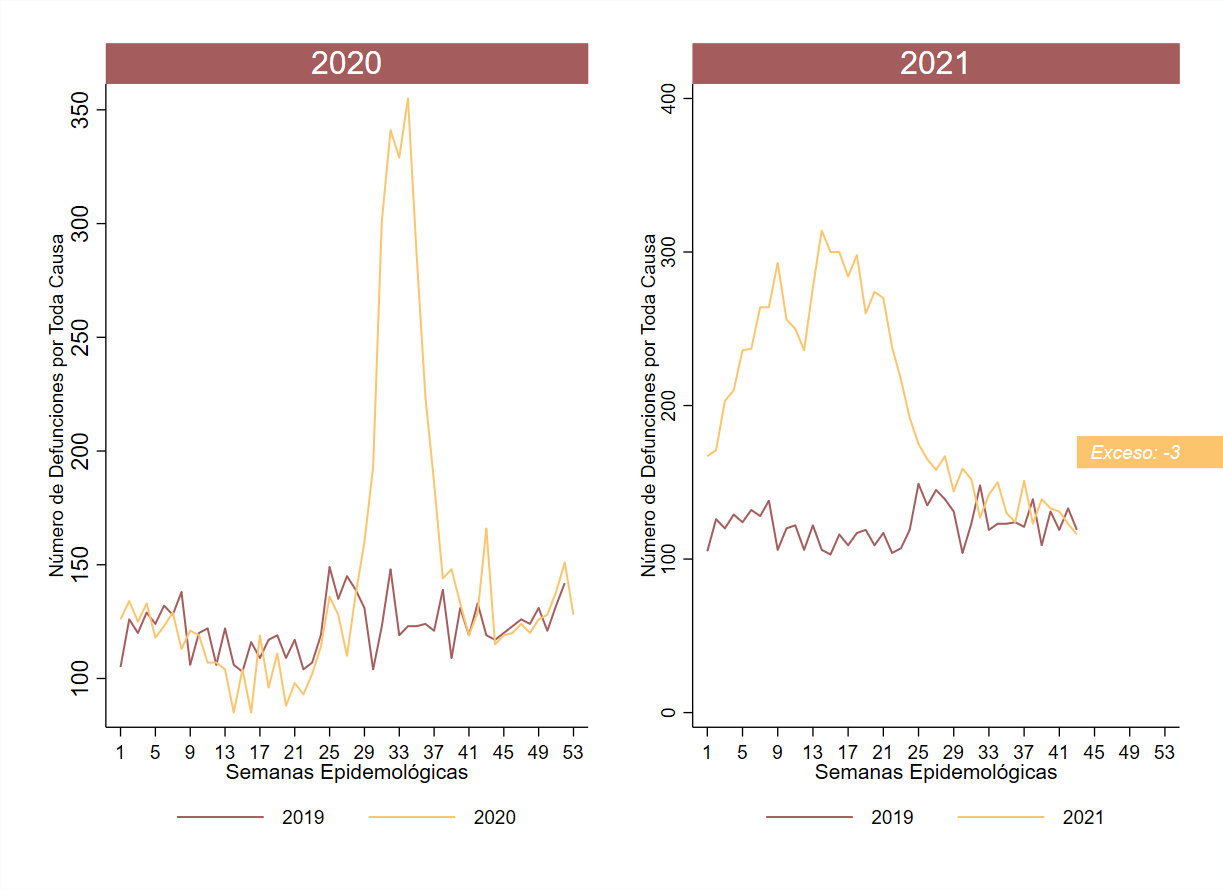
\includegraphics[width=0.65\linewidth]{../figuras/exceso_region}
	\end{center}
	{\footnotesize {Fuente de datos: SISCOVID, NOTICOVID.}}
	\end{figure}

\clearpage
	\section*{Lugar de Ocurrencia de Defunciones por COVID-19}
	\noindent La Figura 15 muestra que del total de fallecidos en la región del Cusco, el 64.1\% de fallecidos por COVID-19 procedieron de tres hospitales: Hospital Nacional Adolfo Guevara Velasco, del Hospital Regional del Cusco( Hospital de Apoyo Departamental), y del Hospital Antonio Lorena. Un 13.2\% de los fallecidos fueron de los Hospitales del II Nivel de atención. Las defunciones extramurales representadas por las defunciones en domicilios, en tránsito y en vía pública por COVID-19, representaron el 18.1\%, porcentaje que aún no ha superado la afección de la primera ola (21\%).

[Insertar figura]

\clearpage
	\section*{Evaluación Provincial de la Infección por COVID-19}
	\noindent El Cuadro \ref{tab:leta_mort_provincial} muestra la tasa de letalidad y mortalidad de todas las provincias de la Región Cusco. Se presentan las provincias ordenadas de mayor a menor tasa de mortalidad. Hasta la SE 33 la provincia con mayor tasa de mortalidad sigue siendo Canchis (271 defunciones por 100,000 habitantes) sin variación con respecto a la publicación del Boletín anterior. En contraste, la mortalidad en Espinar es baja en comparación a las demás provincias (76 defunciones por 100,000 habitantes). La tasa de letalidad, es mayor en las provincias de Paruro, Canas, Canchis y Quispicanchi, haciendo notar la presencia de enfermedad más severa en estas provincias. 

	% Insertar el cuadro
	\begin{tabular}{lccccc}
	\rowcolor[HTML]{DDEBF7} 
	\multicolumn{1}{c}{\cellcolor[HTML]{DDEBF7}\textbf{Provincias}} & \textbf{Población}   & \textbf{Total de  Pruebas} & \textbf{Defunciones} & \textbf{Tasa de letalidad} & \textbf{Tasa de mortalidad x   100,000 hab} \\
	\cellcolor[HTML]{FF5050}CANCHIS                                 & 105,049              & 4,325                      & 291                  & 6.7\%                      & 277.0                                       \\
	\cellcolor[HTML]{FF5050}CUSCO                                   & 463,656              & 41,999                     & 1,220                & 2.9\%                      & 263.1                                       \\
	\cellcolor[HTML]{FF5050}ANTA                                    & 57,731               & 2,358                      & 148                  & 6.3\%                      & 256.4                                       \\
	\cellcolor[HTML]{FF5050}QUISPICANCHI                            & 92,566               & 3,021                      & 218                  & 7.2\%                      & 235.5                                       \\
	\cellcolor[HTML]{F4B084}URUBAMBA                                & 66,439               & 3,153                      & 136                  & 4.3\%                      & 204.7                                       \\
	\cellcolor[HTML]{F4B084}CANAS                                   & 40,420               & 837                        & 67                   & 8.0\%                      & 165.8                                       \\
	\cellcolor[HTML]{F4B084}PARURO                                  & 31,264               & 567                        & 49                   & 8.6\%                      & 156.7                                       \\
	\cellcolor[HTML]{F4B084}LA CONVENCIÓN                           & 185,793              & 10,665                     & 290                  & 2.7\%                      & 156.1                                       \\
	\cellcolor[HTML]{FFE699}CHUMBIVILCAS                            & 84,925               & 1,976                      & 108                  & 5.5\%                      & 127.2                                       \\
	\cellcolor[HTML]{FFE699}PAUCARTAMBO                             & 52,989               & 949                        & 67                   & 7.1\%                      & 126.4                                       \\
	\cellcolor[HTML]{FFE699}ACOMAYO                                 & 28,477               & 706                        & 33                   & 4.7\%                      & 115.9                                       \\
	\cellcolor[HTML]{FFE699}CALCA                                   & 76,462               & 1,828                      & 74                   & 4.0\%                      & 96.8                                        \\
	\cellcolor[HTML]{FFE699}ESPINAR                                 & 71,304               & 2,075                      & 55                   & 2.7\%                      & 77.1                                        \\
	& \multicolumn{1}{l}{} & \multicolumn{1}{l}{}       & \multicolumn{1}{l}{} & \multicolumn{1}{l}{}       & \multicolumn{1}{l}{}                        \\
	\rowcolor[HTML]{DDEBF7} 
	\textbf{Total general}                                          & \textbf{1,357,075}   & \textbf{74,459}            & \textbf{2,756}       & \textbf{3.7\%}             & \textbf{203.1}                             
\end{tabular}
 
	{\footnotesize Fuente de datos: NOTICOVID, SISCOVID, SINADEF.}

%---------------------------------------------------------------------------
% CAPÍTULO: EVALUACIÓN DE PROVINCIAS
%---------------------------------------------------------------------------
	\chapter*{Evaluación para Provincias Priorizadas}
	\addcontentsline{toc}{chapter}{Evaluación para Provincias Priorizadas}
	\noindent La Figura \ref{fig:incidencia_provincias} muestra la tendencia de la incidencia provincial de COVID-19. Hasta el 25 de septiembre, término de la SE38, la Provincia de Cusco ha reportado una tendencia levemente creciente de casos. La tendencia de la tasa de incidencia tiene poco crecimiento estas últimas semanas en las demás provincias.
	
	\begin{figure}[h]
		\caption{Tendencia Provincial de Incidencia Acumulada de COVID-19, hasta la SE 38, 2021}\label{fig:incidencia_provincias}
		\begin{center}
			\includegraphics[width=0.65\linewidth]{../figuras/figura16}
		\end{center}
		{\footnotesize {Fuente de datos: SISCOVID, NOTICOVID.}}
	\end{figure}
	
	De la misma forma, la Figura \ref{fig:mortalidad_provincias} muestra la tendencia de la tasa de mortalidad por COVID-19 a nivel provincial. Es así que, la provincia con mayor tasa de mortalidad por esta enfermedad infecciosa es Canchis, al igual que la anterior edición de este Boletín. Las siguientes provincias con más alta tasa de mortalidad son Anta seguida por Cusco. La tendencia de mortalidad en todas las provincias ha crecido poco estas últimas semanas.
	
	En contraste, las provincias con menor tasa de mortalidad fueron Paucartambo, Paruro, Espinar, y Calca. Las demás provincias están entre estos dos grupos.
	
	\begin{figure}[h]
		\caption{Tendencia Provincial de Incidencia acumulada de COVID-19, hasta la SE 38, 2021}\label{fig:mortalidad_provincias}
		\begin{center}
			\includegraphics[width=0.65\linewidth]{../figuras/figura17}
		\end{center}
		{\footnotesize {Fuente de datos: SINADEF.}}
	\end{figure}
	
	\newpage
	
	\section*{Evaluación Provincial de 5 Indicadores}
	\noindent El objetivo de estas figuras es comparar a cada provincia consigo misma de acuerdo a su historia  en la primera ola (en el año 2020). Se evaluaron los siguientes indicadores: incidencia, tasa de mortalidad, tasa de positividad molecular, tasa de positividad antigénica, y exceso de defunciones para cada provincia.
	
	\subsection*{Provincia de Acomayo}
	\noindent Las figuras inferiores (Figura \ref{fig:inc_mort_acomayo}, \ref{fig:positividad_acomayo}) muestran una importante disminución de la mortalidad e incidencia en estas últimas semanas, siendo mayor a partir de la SE 20. La tasa de positividad molecular y antigénica disminuyeron en las últimas semanas. En la Figura \ref{fig:exceso_acomayo} se muestra que no hay exceso de defunciones respecto al año 2019.
	
	\begin{figure}[h]
		\caption{Tasa de Incidencia y Mortalidad Comparativa en la Provincia de Acomayo 2020 y 2021, hasta la SE 38}\label{fig:inc_mort_acomayo}
		\begin{center}
			\includegraphics[width=0.7\linewidth]{../figuras/provincia_m1}
		\end{center}
		{\footnotesize {Fuente de datos: NOTICOVID, SISCOVID, SINADEF.}}
	\end{figure}

	\begin{figure}[h]
	\caption{Tasa de Positividad de Prueba Molecular y Antigénica Comparativa en la Provincia de Acomayo 2020 y 2021, hasta la SE 38}\label{fig:positividad_acomayo}
	\begin{center}
		\includegraphics[width=0.7\linewidth]{../figuras/provincia_p1}
	\end{center}
	{\footnotesize {Fuente de datos: NOTICOVID, SISCOVID.}}
	\end{figure}

	\begin{figure}[h]
	\caption{Exceso de Defunciones Comparativo en la Provincia de Acomayo 2019, 2020 y 2021, hasta la SE 38}\label{fig:exceso_acomayo}
	\begin{center}
		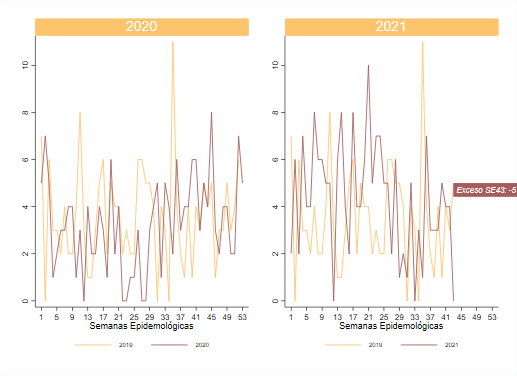
\includegraphics[width=0.7\linewidth]{../figuras/exceso_1}
	\end{center}
	{\footnotesize {Fuente de datos: SINADEF.}}
	\end{figure}

	% Anta
	\clearpage
	
	\subsection*{Provincia de Anta}
	\noindent Las figuras de abajo (Figura \ref{fig:inc_mort_anta}, \ref{fig:positividad_anta})  muestran una disminución importante desde la SE13 en la tasa de mortalidad, que aunque aumentó desde la SE33, llegó a ser bastante baja en la SE38. Similarmente, la tasa de incidencia tiene una caída más sostenida. Hay un pequeño aumento en la tasa de positividad de pruebas moleculares similar a la de pruebas antigénicas estas últimas semanas. En la Figura \ref{fig:exceso_anta} se muestra que no hay exceso de defunciones respecto al año 2019.
	
		\begin{figure}[h]
		\caption{Tasa de Incidencia y Mortalidad Comparativa en la Provincia de Anta 2020 y 2021, hasta la SE 38}\label{fig:inc_mort_anta}
		\begin{center}
			\includegraphics[width=0.7\linewidth]{../figuras/provincia_m2}
		\end{center}
		{\footnotesize {Fuente de datos: NOTICOVID, SISCOVID, SINADEF.}}
	\end{figure}
	
	\begin{figure}[h]
		\caption{Tasa de Positividad de Prueba Molecular y Antigénica Comparativa en la Provincia de Anta 2020 y 2021, hasta la SE 38}\label{fig:positividad_anta}
		\begin{center}
			\includegraphics[width=0.7\linewidth]{../figuras/provincia_p2}
		\end{center}
		{\footnotesize {Fuente de datos: NOTICOVID, SISCOVID.}}
	\end{figure}
	
	\begin{figure}[h]
		\caption{Exceso de Defunciones Comparativo en la Provincia de Anta 2019, 2020 y 2021, hasta la SE 38}\label{fig:exceso_anta}
		\begin{center}
			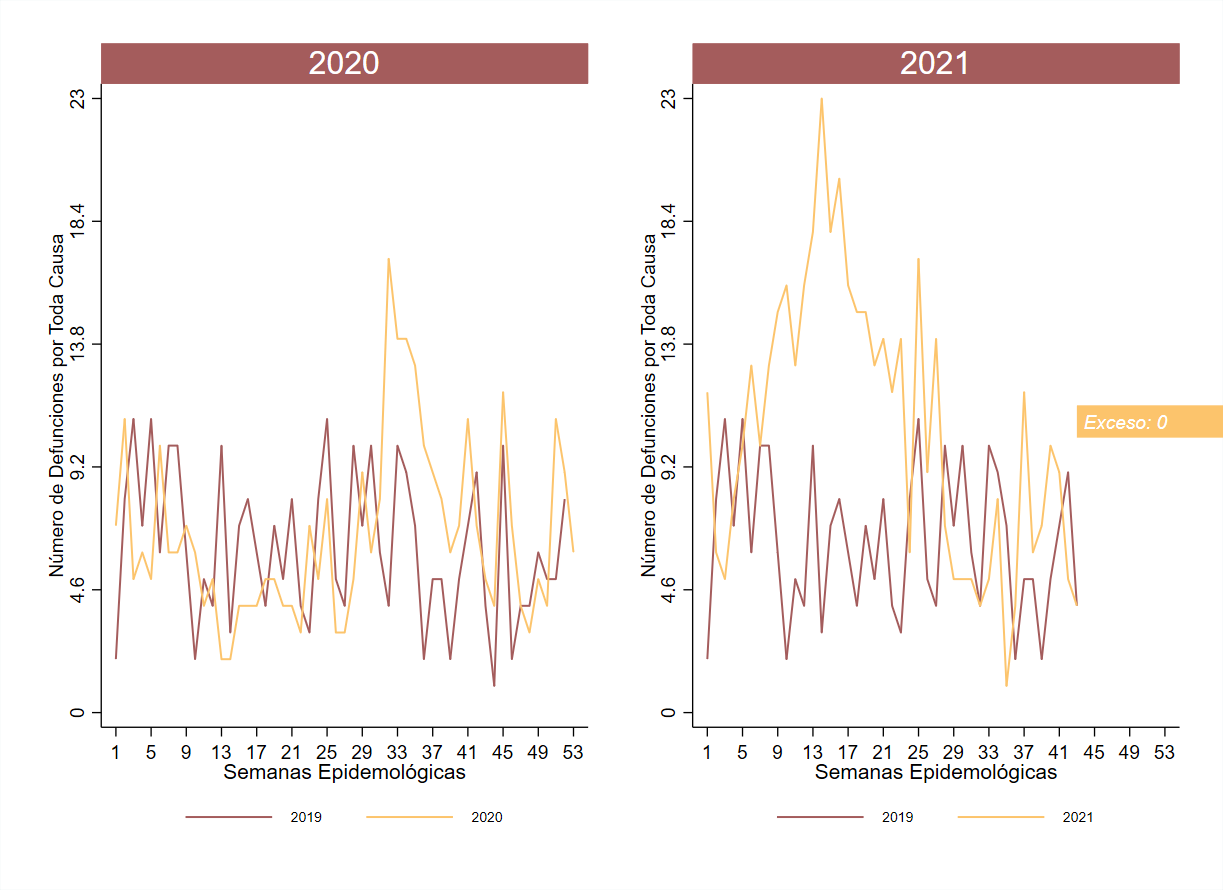
\includegraphics[width=0.7\linewidth]{../figuras/exceso_2}
		\end{center}
		{\footnotesize {Fuente de datos: SINADEF.}}
	\end{figure}

	% Canas
		\clearpage
	
	\subsection*{Provincia de Canas}
	\noindent Las figuras de abajo (Figura \ref{fig:inc_mort_canas}, \ref{fig:positividad_canas})  muestran una disminución importante desde la SE13 en la tasa de mortalidad, que aunque aumentó desde la SE33, llegó a ser bastante baja en la SE38. Similarmente, la tasa de incidencia tiene una caída más sostenida. Hay un pequeño aumento en la tasa de positividad de pruebas moleculares similar a la de pruebas antigénicas estas últimas semanas. En la Figura \ref{fig:exceso_canas} se muestra que no hay exceso de defunciones respecto al año 2019.
	
	\begin{figure}[h]
		\caption{Tasa de Incidencia y Mortalidad Comparativa en la Provincia de Canas 2020 y 2021, hasta la SE 38}\label{fig:inc_mort_canas}
		\begin{center}
			\includegraphics[width=0.7\linewidth]{../figuras/provincia_m3}
		\end{center}
		{\footnotesize {Fuente de datos: NOTICOVID, SISCOVID, SINADEF.}}
	\end{figure}
	
	\begin{figure}[h]
		\caption{Tasa de Positividad de Prueba Molecular y Antigénica Comparativa en la Provincia de Canas 2020 y 2021, hasta la SE 38}\label{fig:positividad_canas}
		\begin{center}
			\includegraphics[width=0.7\linewidth]{../figuras/provincia_p3}
		\end{center}
		{\footnotesize {Fuente de datos: NOTICOVID, SISCOVID.}}
	\end{figure}
	
	\begin{figure}[h]
		\caption{Exceso de Defunciones Comparativo en la Provincia de Canas 2019, 2020 y 2021, hasta la SE 38}\label{fig:exceso_canas}
		\begin{center}
			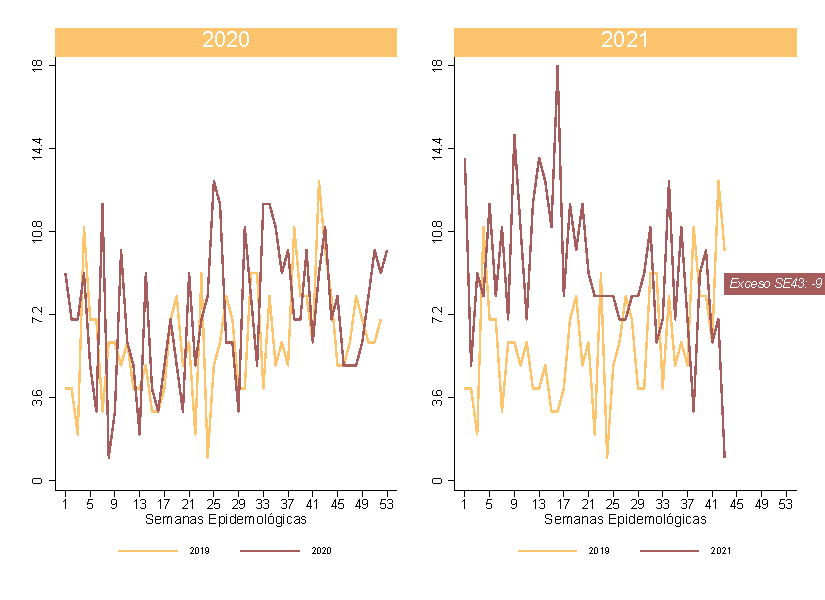
\includegraphics[width=0.7\linewidth]{../figuras/exceso_3}
		\end{center}
		{\footnotesize {Fuente de datos: SINADEF.}}
	\end{figure}

	% Calca
\clearpage

	\subsection*{Provincia de Calca}
	\noindent Las figuras de abajo (Figura \ref{fig:inc_mort_calca}, \ref{fig:positividad_calca})  muestran una disminución importante desde la SE13 en la tasa de mortalidad, que aunque aumentó desde la SE33, llegó a ser bastante baja en la SE38. Similarmente, la tasa de incidencia tiene una caída más sostenida. Hay un pequeño aumento en la tasa de positividad de pruebas moleculares similar a la de pruebas antigénicas estas últimas semanas. En la Figura \ref{fig:exceso_calca} se muestra que no hay exceso de defunciones respecto al año 2019.

	\begin{figure}[h]
	\caption{Tasa de Incidencia y Mortalidad Comparativa en la Provincia de Canas 2020 y 2021, hasta la SE 38}\label{fig:inc_mort_calca}
	\begin{center}
		\includegraphics[width=0.7\linewidth]{../figuras/provincia_m4}
	\end{center}
	{\footnotesize {Fuente de datos: NOTICOVID, SISCOVID, SINADEF.}}
	\end{figure}

	\begin{figure}[h]
	\caption{Tasa de Positividad de Prueba Molecular y Antigénica Comparativa en la Provincia de Canas 2020 y 2021, hasta la SE 38}\label{fig:positividad_calca}
	\begin{center}
		\includegraphics[width=0.7\linewidth]{../figuras/provincia_p4}
	\end{center}
	{\footnotesize {Fuente de datos: NOTICOVID, SISCOVID.}}
	\end{figure}

	\begin{figure}[h]
	\caption{Exceso de Defunciones Comparativo en la Provincia de Canas 2019, 2020 y 2021, hasta la SE 38}\label{fig:exceso_calca}
	\begin{center}
		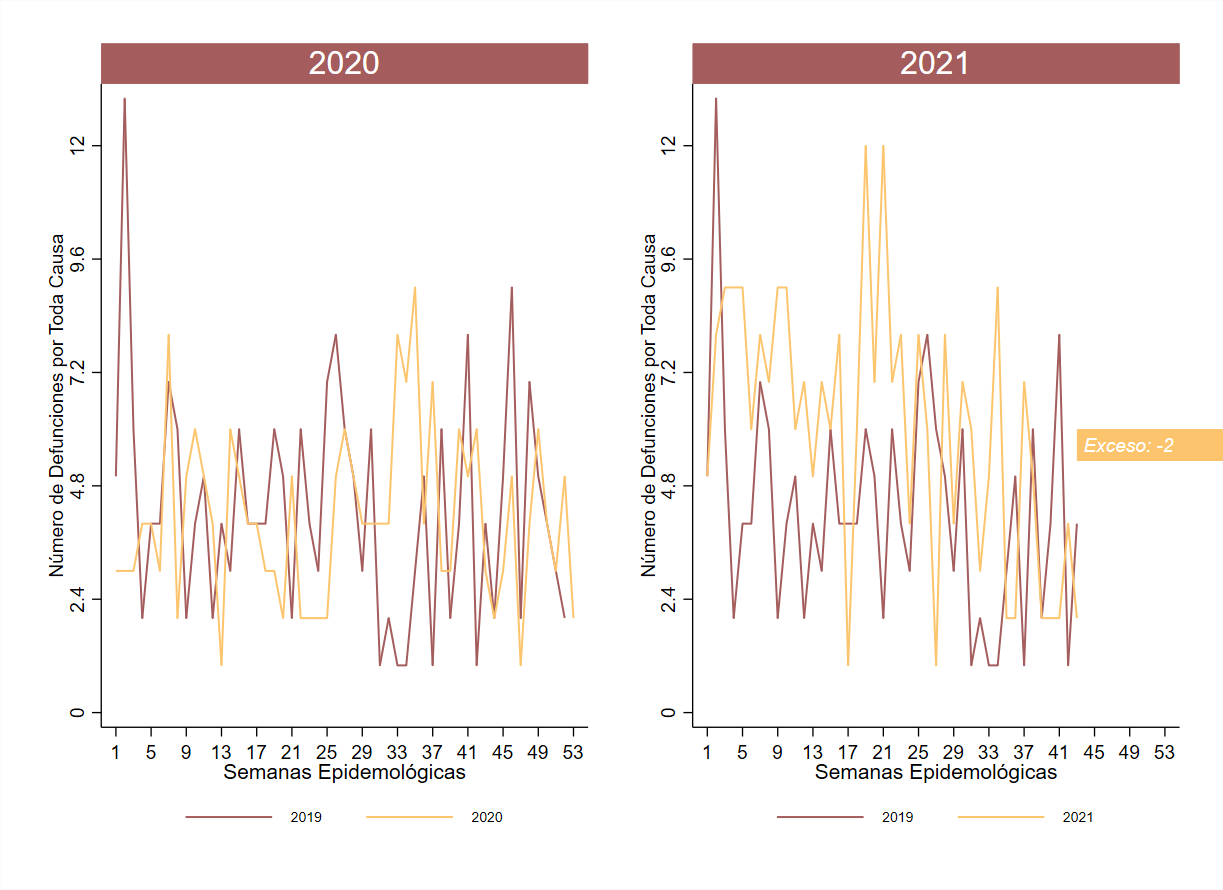
\includegraphics[width=0.7\linewidth]{../figuras/exceso_4}
	\end{center}
	{\footnotesize {Fuente de datos: SINADEF.}}
	\end{figure}

	% Canas
\clearpage

	\subsection*{Provincia de Canchis}
	\noindent Las figuras de abajo (Figura \ref{fig:inc_mort_canchis}, \ref{fig:positividad_canchis})  muestran una disminución importante desde la SE13 en la tasa de mortalidad, que aunque aumentó desde la SE33, llegó a ser bastante baja en la SE38. Similarmente, la tasa de incidencia tiene una caída más sostenida. Hay un pequeño aumento en la tasa de positividad de pruebas moleculares similar a la de pruebas antigénicas estas últimas semanas. En la Figura \ref{fig:exceso_canchis} se muestra que no hay exceso de defunciones respecto al año 2019.

	\begin{figure}[h]
	\caption{Tasa de Incidencia y Mortalidad Comparativa en la Provincia de Canas 2020 y 2021, hasta la SE 38}\label{fig:inc_mort_canchis}
	\begin{center}
		\includegraphics[width=0.7\linewidth]{../figuras/provincia_m5}
	\end{center}
	{\footnotesize {Fuente de datos: NOTICOVID, SISCOVID, SINADEF.}}
	\end{figure}

	\begin{figure}[h]
	\caption{Tasa de Positividad de Prueba Molecular y Antigénica Comparativa en la Provincia de Canas 2020 y 2021, hasta la SE 38}\label{fig:positividad_canchis}
	\begin{center}
		\includegraphics[width=0.7\linewidth]{../figuras/provincia_p5}
	\end{center}
	{\footnotesize {Fuente de datos: NOTICOVID, SISCOVID.}}
	\end{figure}
	
	\begin{figure}[h]
	\caption{Exceso de Defunciones Comparativo en la Provincia de Canas 2019, 2020 y 2021, hasta la SE 38}\label{fig:exceso_canchis}
	\begin{center}
		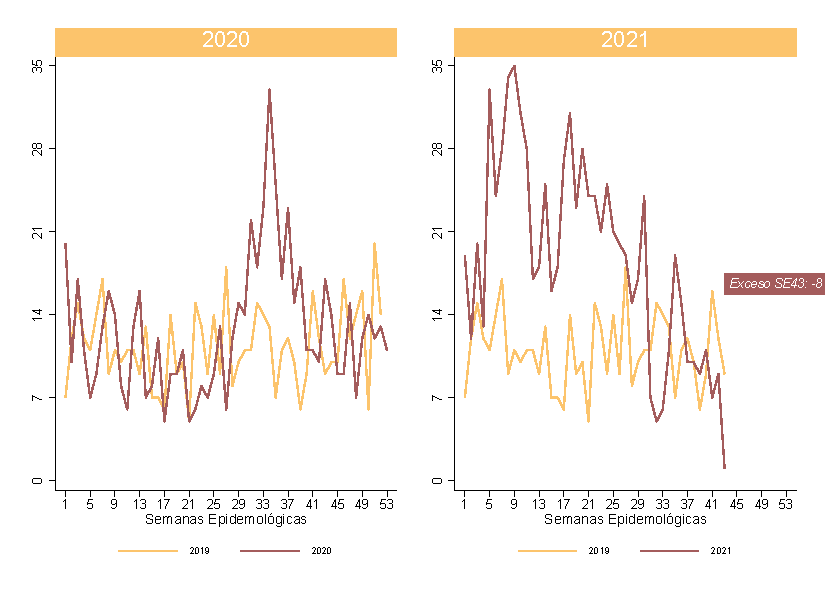
\includegraphics[width=0.7\linewidth]{../figuras/exceso_5}
	\end{center}
	{\footnotesize {Fuente de datos: SINADEF.}}
	\end{figure}

\clearpage

	% Chumbivilcas
	\subsection*{Provincia de Chumbivilcas}
	\noindent Las figuras de abajo (Figura \ref{fig:inc_mort_chumbivilcas}, \ref{fig:positividad_chumbivilcas})  muestran una disminución importante desde la SE13 en la tasa de mortalidad, que aunque aumentó desde la SE33, llegó a ser bastante baja en la SE38. Similarmente, la tasa de incidencia tiene una caída más sostenida. Hay un pequeño aumento en la tasa de positividad de pruebas moleculares similar a la de pruebas antigénicas estas últimas semanas. En la Figura \ref{fig:exceso_chumbivilcas} se muestra que no hay exceso de defunciones respecto al año 2019.

	\begin{figure}[h]
	\caption{Tasa de Incidencia y Mortalidad Comparativa en la Provincia de Chumbivilcas 2020 y 2021, hasta la SE 38}\label{fig:inc_mort_chumbivilcas}
	\begin{center}
		\includegraphics[width=0.7\linewidth]{../figuras/provincia_m6}
	\end{center}
	{\footnotesize {Fuente de datos: NOTICOVID, SISCOVID, SINADEF.}}
	\end{figure}

	\begin{figure}[h]
	\caption{Tasa de Positividad de Prueba Molecular y Antigénica Comparativa en la Provincia de Chumbivilcas 2020 y 2021, hasta la SE 38}\label{fig:positividad_chumbivilcas}
	\begin{center}
		\includegraphics[width=0.7\linewidth]{../figuras/provincia_p6}
	\end{center}
	{\footnotesize {Fuente de datos: NOTICOVID, SISCOVID.}}
	\end{figure}

	\begin{figure}[h]
	\caption{Exceso de Defunciones Comparativo en la Provincia de Chumbivilcas 2019, 2020 y 2021, hasta la SE 38}\label{fig:exceso_chumbivilcas}
	\begin{center}
		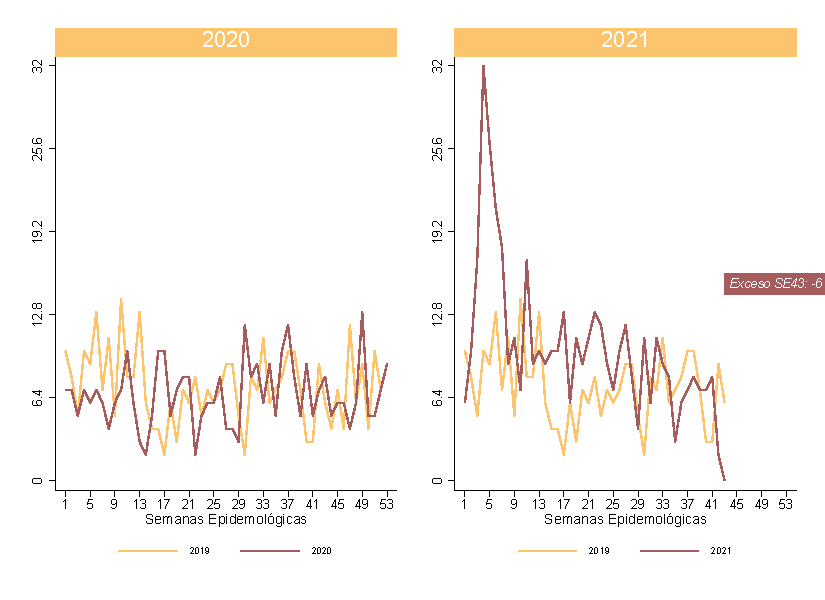
\includegraphics[width=0.7\linewidth]{../figuras/exceso_6}
	\end{center}
	{\footnotesize {Fuente de datos: SINADEF.}}
	\end{figure}

% Cusco
\clearpage

	\subsection*{Provincia de Cusco}
	\noindent Las figuras de abajo (Figura \ref{fig:inc_mort_cusco}, \ref{fig:positividad_cusco})  muestran una disminución importante desde la SE13 en la tasa de mortalidad, que aunque aumentó desde la SE33, llegó a ser bastante baja en la SE38. Similarmente, la tasa de incidencia tiene una caída más sostenida. Hay un pequeño aumento en la tasa de positividad de pruebas moleculares similar a la de pruebas antigénicas estas últimas semanas. En la Figura \ref{fig:exceso_cusco} se muestra que no hay exceso de defunciones respecto al año 2019.

	\begin{figure}[h]
	\caption{Tasa de Incidencia y Mortalidad Comparativa en la Provincia de Cusco 2020 y 2021, hasta la SE 38}\label{fig:inc_mort_cusco}
	\begin{center}
		\includegraphics[width=0.7\linewidth]{../figuras/provincia_m7}
	\end{center}
	{\footnotesize {Fuente de datos: NOTICOVID, SISCOVID, SINADEF.}}
	\end{figure}

	\begin{figure}[h]
	\caption{Tasa de Positividad de Prueba Molecular y Antigénica Comparativa en la Provincia de Cusco 2020 y 2021, hasta la SE 38}\label{fig:positividad_cusco}
	\begin{center}
		\includegraphics[width=0.7\linewidth]{../figuras/provincia_p7}
	\end{center}
	{\footnotesize {Fuente de datos: NOTICOVID, SISCOVID.}}
	\end{figure}

	\begin{figure}[h]
	\caption{Exceso de Defunciones Comparativo en la Provincia de Cusco 2019, 2020 y 2021, hasta la SE 38}\label{fig:exceso_cusco}
	\begin{center}
		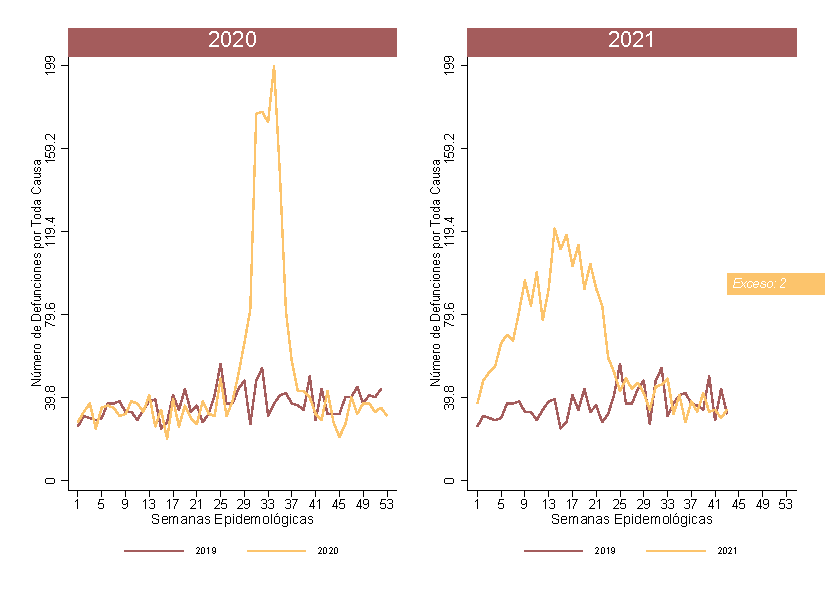
\includegraphics[width=0.7\linewidth]{../figuras/exceso_7}
	\end{center}
	{\footnotesize {Fuente de datos: SINADEF.}}
	\end{figure}

% Espinar
\clearpage

	\subsection*{Provincia de Espinar}
	\noindent Las figuras de abajo (Figura \ref{fig:inc_mort_espinar}, \ref{fig:positividad_espinar})  muestran una disminución importante desde la SE13 en la tasa de mortalidad, que aunque aumentó desde la SE33, llegó a ser bastante baja en la SE38. Similarmente, la tasa de incidencia tiene una caída más sostenida. Hay un pequeño aumento en la tasa de positividad de pruebas moleculares similar a la de pruebas antigénicas estas últimas semanas. En la Figura \ref{fig:exceso_espinar} se muestra que no hay exceso de defunciones respecto al año 2019.

	\begin{figure}[h]
	\caption{Tasa de Incidencia y Mortalidad Comparativa en la Provincia de Espinar 2020 y 2021, hasta la SE 38}\label{fig:inc_mort_espinar}
	\begin{center}
		\includegraphics[width=0.7\linewidth]{../figuras/provincia_m8}
	\end{center}
	{\footnotesize {Fuente de datos: NOTICOVID, SISCOVID, SINADEF.}}
	\end{figure}

	\begin{figure}[h]
	\caption{Tasa de Positividad de Prueba Molecular y Antigénica Comparativa en la Provincia de Espinar 2020 y 2021, hasta la SE 38}\label{fig:positividad_espinar}
	\begin{center}
		\includegraphics[width=0.7\linewidth]{../figuras/provincia_p8}
	\end{center}
	{\footnotesize {Fuente de datos: NOTICOVID, SISCOVID.}}
	\end{figure}

	\begin{figure}[h]
	\caption{Exceso de Defunciones Comparativo en la Provincia de Espinar 2019, 2020 y 2021, hasta la SE 38}\label{fig:exceso_espinar}
	\begin{center}
		\includegraphics[width=0.7\linewidth]{../figuras/exceso_8}
	\end{center}
	{\footnotesize {Fuente de datos: SINADEF.}}
	\end{figure}

% La Convención
\clearpage

	\subsection*{Provincia de La Convención}
	\noindent Las figuras de abajo (Figura \ref{fig:inc_mort_laconv}, \ref{fig:positividad_laconv})  muestran una disminución importante desde la SE13 en la tasa de mortalidad, que aunque aumentó desde la SE33, llegó a ser bastante baja en la SE38. Similarmente, la tasa de incidencia tiene una caída más sostenida. Hay un pequeño aumento en la tasa de positividad de pruebas moleculares similar a la de pruebas antigénicas estas últimas semanas. En la Figura \ref{fig:exceso_laconv} se muestra que no hay exceso de defunciones respecto al año 2019.

	\begin{figure}[h]
	\caption{Tasa de Incidencia y Mortalidad Comparativa en la Provincia de La Convención 2020 y 2021, hasta la SE 38}\label{fig:inc_mort_laconv}
	\begin{center}
		\includegraphics[width=0.7\linewidth]{../figuras/provincia_m9}
	\end{center}
	{\footnotesize {Fuente de datos: NOTICOVID, SISCOVID, SINADEF.}}
	\end{figure}

	\begin{figure}[h]
	\caption{Tasa de Positividad de Prueba Molecular y Antigénica Comparativa en la Provincia de La Convención 2020 y 2021, hasta la SE 38}\label{fig:positividad_laconv}
	\begin{center}
		\includegraphics[width=0.7\linewidth]{../figuras/provincia_p9}
	\end{center}
	{\footnotesize {Fuente de datos: NOTICOVID, SISCOVID.}}
	\end{figure}

	\begin{figure}[h]
	\caption{Exceso de Defunciones Comparativo en la Provincia de La Convención 2019, 2020 y 2021, hasta la SE 38}\label{fig:exceso_laconv}
	\begin{center}
		\includegraphics[width=0.7\linewidth]{../figuras/exceso_9}
	\end{center}
	{\footnotesize {Fuente de datos: SINADEF.}}
	\end{figure}

% Paruro
\clearpage

	\subsection*{Provincia de Paruro}
	\noindent Las figuras de abajo (Figura \ref{fig:inc_mort_paruro}, \ref{fig:positividad_paruro})  muestran una disminución importante desde la SE13 en la tasa de mortalidad, que aunque aumentó desde la SE33, llegó a ser bastante baja en la SE38. Similarmente, la tasa de incidencia tiene una caída más sostenida. Hay un pequeño aumento en la tasa de positividad de pruebas moleculares similar a la de pruebas antigénicas estas últimas semanas. En la Figura \ref{fig:exceso_paruro} se muestra que no hay exceso de defunciones respecto al año 2019.

	\begin{figure}[h]
	\caption{Tasa de Incidencia y Mortalidad Comparativa en la Provincia de Paruro 2020 y 2021, hasta la SE 38}\label{fig:inc_mort_paruro}
	\begin{center}
		\includegraphics[width=0.7\linewidth]{../figuras/provincia_m10}
	\end{center}
	{\footnotesize {Fuente de datos: NOTICOVID, SISCOVID, SINADEF.}}
	\end{figure}

	\begin{figure}[h]
	\caption{Tasa de Positividad de Prueba Molecular y Antigénica Comparativa en la Provincia de Paruro 2020 y 2021, hasta la SE 38}\label{fig:positividad_paruro}
	\begin{center}
		\includegraphics[width=0.7\linewidth]{../figuras/provincia_p10}
	\end{center}
	{\footnotesize {Fuente de datos: NOTICOVID, SISCOVID.}}
	\end{figure}

	\begin{figure}[h]
	\caption{Exceso de Defunciones Comparativo en la Provincia de Paruro 2019, 2020 y 2021, hasta la SE 38}\label{fig:exceso_paruro}
	\begin{center}
		\includegraphics[width=0.7\linewidth]{../figuras/exceso_10}
	\end{center}
	{\footnotesize {Fuente de datos: SINADEF.}}
	\end{figure}


% Paucartambo
\clearpage

	\subsection*{Provincia de Paucartambo}
	\noindent Las figuras de abajo (Figura \ref{fig:inc_mort_paucartam}, \ref{fig:positividad_paucartam})  muestran una disminución importante desde la SE13 en la tasa de mortalidad, que aunque aumentó desde la SE33, llegó a ser bastante baja en la SE38. Similarmente, la tasa de incidencia tiene una caída más sostenida. Hay un pequeño aumento en la tasa de positividad de pruebas moleculares similar a la de pruebas antigénicas estas últimas semanas. En la Figura \ref{fig:exceso_paucartam} se muestra que no hay exceso de defunciones respecto al año 2019.

	\begin{figure}[h]
	\caption{Tasa de Incidencia y Mortalidad Comparativa en la Provincia de Paucartambo 2020 y 2021, hasta la SE 38}\label{fig:inc_mort_paucartam}
	\begin{center}
		\includegraphics[width=0.7\linewidth]{../figuras/provincia_m11}
	\end{center}
	{\footnotesize {Fuente de datos: NOTICOVID, SISCOVID, SINADEF.}}
	\end{figure}

	\begin{figure}[h]
	\caption{Tasa de Positividad de Prueba Molecular y Antigénica Comparativa en la Provincia de Paucartambo 2020 y 2021, hasta la SE 38}\label{fig:positividad_paucartam}
	\begin{center}
		\includegraphics[width=0.7\linewidth]{../figuras/provincia_p11}
	\end{center}
	{\footnotesize {Fuente de datos: NOTICOVID, SISCOVID.}}
	\end{figure}

	\begin{figure}[h]
	\caption{Exceso de Defunciones Comparativo en la Provincia de Paucartambo 2019, 2020 y 2021, hasta la SE 38}\label{fig:exceso_paucartam}
	\begin{center}
		\includegraphics[width=0.7\linewidth]{../figuras/exceso_11}
	\end{center}
	{\footnotesize {Fuente de datos: SINADEF.}}
	\end{figure}

% Quispicanchi
\clearpage

	\subsection*{Provincia de Quispicanchi}
	\noindent Las figuras de abajo (Figura \ref{fig:inc_mort_quisp}, \ref{fig:positividad_quisp})  muestran una disminución importante desde la SE13 en la tasa de mortalidad, que aunque aumentó desde la SE33, llegó a ser bastante baja en la SE38. Similarmente, la tasa de incidencia tiene una caída más sostenida. Hay un pequeño aumento en la tasa de positividad de pruebas moleculares similar a la de pruebas antigénicas estas últimas semanas. En la Figura \ref{fig:exceso_quisp} se muestra que no hay exceso de defunciones respecto al año 2019.

	\begin{figure}[h]
	\caption{Tasa de Incidencia y Mortalidad Comparativa en la Provincia de Quispicanchi 2020 y 2021, hasta la SE 38}\label{fig:inc_mort_quisp}
	\begin{center}
		\includegraphics[width=0.7\linewidth]{../figuras/provincia_m12}
	\end{center}
	{\footnotesize {Fuente de datos: NOTICOVID, SISCOVID, SINADEF.}}
	\end{figure}

	\begin{figure}[h]
	\caption{Tasa de Positividad de Prueba Molecular y Antigénica Comparativa en la Provincia de Quispicanchi 2020 y 2021, hasta la SE 38}\label{fig:positividad_quisp}
	\begin{center}
		\includegraphics[width=0.7\linewidth]{../figuras/provincia_p12}
	\end{center}
	{\footnotesize {Fuente de datos: NOTICOVID, SISCOVID.}}
	\end{figure}

	\begin{figure}[h]
	\caption{Exceso de Defunciones Comparativo en la Provincia de Quispicanchi 2019, 2020 y 2021, hasta la SE 38}\label{fig:exceso_quisp}
	\begin{center}
		\includegraphics[width=0.7\linewidth]{../figuras/exceso_12}
	\end{center}
	{\footnotesize {Fuente de datos: SINADEF.}}
	\end{figure}

% Urubamba
\clearpage

	\subsection*{Provincia de Urubamba}
	\noindent Las figuras de abajo (Figura \ref{fig:inc_urub}, \ref{fig:positividad_urub})  muestran una disminución importante desde la SE13 en la tasa de mortalidad, que aunque aumentó desde la SE33, llegó a ser bastante baja en la SE38. Similarmente, la tasa de incidencia tiene una caída más sostenida. Hay un pequeño aumento en la tasa de positividad de pruebas moleculares similar a la de pruebas antigénicas estas últimas semanas. En la Figura \ref{fig:exceso_urub} se muestra que no hay exceso de defunciones respecto al año 2019.

	\begin{figure}[h]
	\caption{Tasa de Incidencia y Mortalidad Comparativa en la Provincia de Urubamba 2020 y 2021, hasta la SE 38}\label{fig:inc_urub}
	\begin{center}
		\includegraphics[width=0.7\linewidth]{../figuras/provincia_m13}
	\end{center}
	{\footnotesize {Fuente de datos: NOTICOVID, SISCOVID, SINADEF.}}
	\end{figure}

	\begin{figure}[h]
	\caption{Tasa de Positividad de Prueba Molecular y Antigénica Comparativa en la Provincia de Urubamba 2020 y 2021, hasta la SE 38}\label{fig:positividad_urub}
	\begin{center}
		\includegraphics[width=0.7\linewidth]{../figuras/provincia_p13}
	\end{center}
	{\footnotesize {Fuente de datos: NOTICOVID, SISCOVID.}}
	\end{figure}

	\begin{figure}[h]
	\caption{Exceso de Defunciones Comparativo en la Provincia de Urubamba 2019, 2020 y 2021, hasta la SE 38}\label{fig:exceso_urub}
	\begin{center}
		\includegraphics[width=0.7\linewidth]{../figuras/exceso_13}
	\end{center}
	{\footnotesize {Fuente de datos: SINADEF.}}
	\end{figure}
%---------------------------------------------------------------------------
% CAPÍTULO: VARIANTES DE COVID-19
%---------------------------------------------------------------------------
	\chapter*{Variantes de COVID-19}
	\addcontentsline{toc}{chapter}{Variantes de COVID-19}
	\noindent Las variantes genéticas del SARS-CoV-2 han estado emergiendo y circulando por el mundo durante toda la pandemia del COVID-19. Las variantes y mutaciones virales en la región Cusco son monitoreadas de forma rutinaria mediante la vigilancia secuencial realizada por el laboratorio referencial del Instituto Nacional de Salud. Asimismo, hasta la fecha se ha tenido la colaboración de la Universidad Nacional de San Antonio Abad del Cusco y de la Universidad Peruana Cayetano Heredia, con las que se ha realizado investigaciones epidemiológicas de secuenciamiento viral en SARS-CoV-2.
	
	A nivel de la región Cusco hasta la SE 38,  se realizó el secuenciamiento genético a 262 pruebas positivas para COVID-19, en la Figura 31C se muestra el porcentaje (\%) de cada variante encontrada. Se observa que la variante más prevalente (78.49\%) corresponde a la variante Lambda, seguida de la variante gamma ( 13.44\%) y en menor proporción las variantes delta (B 1617), B1134 y B 1621.
	
	[Insertar figura]
	
%---------------------------------------------------------------------------
% CAPÍTULO: DEFUNCIONES CERO
%---------------------------------------------------------------------------
	\chapter*{Semanas con Cero Defunciones por COVID-19 por Semana a Nivel Provincial}
	\addcontentsline{toc}{chapter}{Defunciones Cero}
	\noindent En las últimas semanas ha existido un gran interés en la disminución de defunciones por COVID-19 a nivel nacional. Cusco ha experimentado una importante disminución de fallecidos por esta enfermedad.  La siguiente figura (Figura 32) muestra la cantidad de fallecidos por semana epidemiológica. Se muestra el análisis desde la semana 31 a la 38 (del 1 de agosto al 25 de septiembre). Las regiones pintadas de celeste indican cero fallecidos por COVID en la respectiva provincia.
	
	Es interesante notar que existe una disminución de defunciones en todas las provincias en el periodo analizado. Espinar es un caso notable en no reportar defunciones en estas últimas semanas. Aunque la Provincia Cusco siempre ha reportado fallecidos por COVID, ésta ha disminuido a lo largo del periodo analizado. La última semana (SE38) 9 de las 13 provincias reportaron cero defunciones.
	
	[Insertar figura]


%---------------------------------------------------------------------------
% CAPÍTULO: AGRADECIMIENTOS
%---------------------------------------------------------------------------
	\chapter*{Agradecimientos}
	\addcontentsline{toc}{chapter}{Agradecimientos}
		
	\centering
		{\large El presente Boletín Epidemiológico COVID-19 se ha elaborado gracias a la información y esfuerzo conjunto de los Equipos de Inteligencia Sanitaria de los Hospitales y Redes de la GERESA Cusco:

		\vspace{0.5cm}
		\noindent
		\begin{minipage}[t]{.45\textwidth}
			\centering
			Hospital Regional del Cusco \\
			M.S.P. Marina Ochoa Linares \vspace{0.5cm}\\
			Hospital Antonio Lorena \\
			Dr. Rony Monge \vspace{.5cm}\\
			Hospital Nacional Adolfo Guevara Velazco\\
			M.S.P. Lucio Velasquez Cuentas \vspace{.5cm}\\
			Red de Salud Norte \\
			M.C. Guido Giraldo Alencastre\vspace{0.5cm}\\
			Red de Salud Sur\\
			Lic. Luz Marina Bernable Villasante \vspace{0.5cm}\\	
		\end{minipage}
		\hfill
		\noindent
		\begin{minipage}[t]{.45\textwidth}
			\centering
			Red de Salud La Convención\\
			Dr. David Coanqui Pacori\vspace{0.5cm}\\
			Red de Salud Chumbivilcas\\
			Lic. Eduarda Benito Calderón \vspace{.5cm}\\
			Red de Salud Canas Canchis Espinar\\
			MC. William Achahui Mercado \vspace{.5cm}\\
			Red de Salud Kimbiri Pichari \\
			Lic Fiorela Alvarez Nihua\vspace{0.5cm}\\	
		\end{minipage}
%---------------------------------------------------------------------------
% CAPÍTULO: AGRADECIMIENTOS
%---------------------------------------------------------------------------
	\chapter*{Diseño y Edición}
	\addcontentsline{toc}{chapter}{Diseño y Edición}
	\begin{center}
	
	% Como siempre, por orden alfabético del apellido
	\href{https://sites.google.com/view/joharcassa}{Econ. Johar Jurimao Cassa Avendaño}
	
	MSC. Fátima R. Concha Velasco
	
	M.C. Ana Gabriela Eulalia Moncada Arias 
	\end{center}

	%insertar la última página
	\includepdf[pages={1}]{../editorial/pagina_final.pdf}
	\clearpage
	
\end{document}